\chapter{Estado da Arte}
\label{ch::arte}

%\section{Introdução}
%\label{sec::arte:intro}

A visualização computacional de funções é a base de muitas aplicações práticas em computação gráfica, tais como em videojogos e visualização molecular. O estudo destas funções permite igualmente outro tipo de cálculos, tais como colisões.

Para alcançar os objetivos propostos no presente projeto, é imperativo estudar os seguintes tópicos:

\begin{itemize}[nosep]
	\item Funções implícitas;
	\item Técnicas de renderização em geral e algoritmos volumétricos em particular;
	\item Uso da \ac{API} \opengl e programação em \ac{GLSL}.
\end{itemize}


\section{Funções Implícitas}
\label{sec::arte:implicitas}

Às funções definidas em função de uma variável dá-se o nome de \textbf{funções explícitas}. Exemplos clássicos em $\mathbb{R}^2$ incluem equações de retas ($y = mx + b$) e parábolas ($y = ax^2 + bx + c$). Ora, nem todos os subconjuntos de pontos no espaço cartesiano podem ser definidos por funções explícitas. Um exemplo comum em $\mathbb{R}^2$ é a circunferência:

\begin{equation}
	(x - x_0)^2 + (y - y_0)^2 = r^2
	\label{eq::circ_implicita}
\end{equation}

onde $(x_0, y_0)$ é o centro e $r$ o raio. Exemplifica-se na Figura \ref{fig::circumference} a circunferência definida por $(x - 1)^2 + (y - 2)^2 = 4$.

\begin{figure}[!btp]
	\centering
	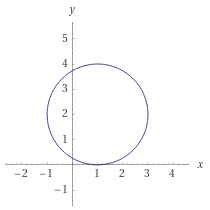
\includegraphics[scale=1.0]{circumference}
	\caption[Exemplo de uma circunferência]{Exemplo de uma circunferência de centro $(1, 2)$ e raio $2$.}
	\label{fig::circumference}
\end{figure}

Sendo uma equação de segundo grau, é possível representá-la através de duas funções explícitas:

\begin{eqnarray}
		y = y_0 + \sqrt{r^2 - (x - x_0)^2} \\
		y = y_0 - \sqrt{r^2 - (x - x_0)^2}
\end{eqnarray}

Esta transformação não é possível para todos os polinómios, em particular para graus superiores a $4$. Contudo, estas expressões polinomiais continuam a ser subconjuntos válidos de $\mathbb{R}^n$, necessitando então de formas alternativas de representação. Dois métodos e respetivas representações da circunferência são:

\begin{enumerate}
	\item \textbf{Funções paramétricas}: cada eixo é definido em ordem a uma variável adicional $t$:
	\begin{equation}
		\left\{\begin{array}{l}
			x = r\cos(t) \\
			y = r\sin(t)
		\end{array}\right.
	\label{eq::circ_parametrica}
	\end{equation}
	
	\item \textbf{Funções implícitas}: a equação não é definida a ordem a uma variável em particular (equação (\ref{eq::circ_implicita})).
\end{enumerate}

Uma \textbf{função implícita} é então definida por $f~:~\mathbb{R}^n \longrightarrow \mathbb{R}$, ou seja, para qualquer ponto em $\mathbb{R}^n$ é determinado um resultado em $\mathbb{R}$. Dependendo da função, o valor obtido pode ter significado, tal como uma grandeza física (\textit{e.g.} densidade de um líquido ou sua temperatura a cada ponto do espaço). Esta função diz-se \textbf{algébrica} caso seja polinomial em cada variável.

Por seu turno, em $\mathbb{R}^3$, a \textbf{iso-superfície} de uma função implícita é a superfície que satisfaz a condição $f(\mathbf{x}) = 0$ (onde, doravante, $\mathbf{x} \equiv (x,y,z)$). Esta pode ser suavizada através de um parâmetro $s \in \mathbb{R}$ tal que:

\begin{equation}
	f(\mathbf{x}) - s = 0
	\label{eq::suavizacao}
\end{equation}

Este efeito é utilizado diretamente e com sucesso nas Superfícies $\Pi$ \cite{Raposo2019}.


\section{Renderização de Superfícies Implícitas}
\label{sec::arte:render}

Muitos algoritmos de renderização têm vindo a ser investigados e usados em \textit{software} que implemente diversas técnicas para obter uma imagem final.

A nossa visão capta a luz refletida por objetos num determinado cenário. Durante o processo, uma parte dos comprimentos de onda das fontes de luz são absorvidos pelos objetos, sendo a restante refletida. Como resultado final, os comprimentos de onda refletidos e captados pelos olhos constituem o que é interpretado pelo cérebro como \textbf{cor}.

No entanto, a determinação do percurso de cada partícula de luz (ou fotão) num dado cenário é na grande maioria dos casos algo impraticável devido ao volume de cálculos envolvidos, com a consequente demora na obtenção dos resultados.

Neste sentido, foram desenvolvidos métodos mais eficientes de cálculo, tais como:

\begin{itemize}
    \item \textbf{Rasterização}: técnica ainda usada na \textit{pipeline} do \opengl, consiste na conversão de uma imagem descrita geometricamente em 3D numa série de pixeis que, no seu todo, criam a sua imagem representativa em 2D;
    
    \item \textbf{\itshape Ray Casting}: considerando um cenário a ser observado a partir de um determinado ponto de vista, este algoritmo calcula a imagem observada com base na geometria e em leis óticas fundamentais;
    
    \item \textbf{\itshape Ray Tracing}: funcionalmente semelhante ao \textit{Ray Casting}, recorre a simulações óticas mais avançadas para a criação de cenários mais realistas.
\end{itemize}

%\todo{Imagens de exemplo de cada técnica.}

Neste âmbito, as funções implícitas representam simultaneamente uma grande oportunidade e um enorme desafio na área da computação gráfica. Se por um lado é possível obter a visualização de formas geométricas complexas com recurso a funções implícitas, por outro não há um método direto geral para determinar os pontos da iso-superfície. Vários algoritmos computacionais para este fim têm sido propostos ao longo das últimas décadas. Para fins do presente Estado da Arte, estes podem ser categorizados em dois grandes grupos:

\begin{enumerate}
	\item \textbf{Triangulação}: A iso-superfície é dividida em triângulos, os quais formam a \textit{mesh} a ser renderizada pela \ac{GPU}. Este é considerado o algoritmo clássico e de eleição:
	\begin{itemize}[nosep]
		\item \textit{Marching cubes}\cite{Lorensen1987}: O espaço é dividido em cubos onde o valor da função implícita é calculado para cada vértice. A análise dos sinais permite determinar quais arestas do cubo a superfície interseta, num total de 256 possíveis combinações de triângulos.
	\end{itemize}
	
	\item \textbf{Algoritmos volumétricos}: Permitem determinar a iso-superfície através do cálculo de interseções. Exemplos incluem:
	\begin{itemize}
		\item \textit{Ray marching}: Uma série finita de raios com origem no observador são emitidos para a cena a ser visualizada, e a interseção é estimada iterando sobre um ponto que marcha nesse raio.
		\item \textit{Sphere tracing}\cite{Hart1996}: Um caso particular de \textit{ray marching} onde esferas são usadas para determinar a distância mínima aos objetos do cenário.
		\item \textit{Ray tracing} (previamente descrito).
	\end{itemize}
\end{enumerate}

%	\item \textbf{\textit{Ray Tracing}}:\\
%    \revision{} \todo{Citar um artigo de Ray Tracing}\\
%     Um \textit{viewport} é definido a uma distância da câmara. É a partir da mesma que são enviados raios na direção de cada pixel. É calculado o ponto de interseção com a superfície em cena e o mesmo é refletido. Este processo é repetido uma quantia pre-definida até por fim obter a cor a usar.


\section{\emph{Ray Marching}}
\label{sec::arte:raymarch}

%\revision{\textit{Ray marching} é uma técnica de renderização que tal como no tradicional \textit{ray tracing}, não é tão simples de resolver uma superfície (ou até impossível caso sem o uso de métodos numéricos interativos). Em \textit{ray tracing} apenas nos focamos na interseção do raio emitido com a superfície, enquanto no algoritmo de \textit{ray marching} marchamos na direção tomada até encontrarmos uma interseção (isto se a mesma existir).}

Um método de estimar pontos da iso-superfície de uma função implícita passa pela determinação da sua interseção com retas. Pelo princípio tomado nos métodos da família de \textit{ray casting}, um raio com origem no observador e um sentido na cena a ser observada é considerado. Diferentes algoritmos podem ser utilizados para estimar o ponto de interseção (ou calcular com precisão se tal for possível). No caso de \textit{ray marching}, a interseção do raio com a superfície implícita é feita colocando um ponto em ``marcha'' ao longo do primeiro.

\subsection{\textit{Ray Casting}}
\label{ssec::arte:raymarch:cast}

Seguir-se-á uma explicação do processo de \textit{ray casting} tendo por base o esquema da Figura \ref{fig::raycast}.

Considere-se então os seguintes parâmetros relativos ao \textbf{observador} (ou câmara):

\begin{itemize}
	\item \textbf{Origem} no ponto $C$;
	\item \textbf{Vetores de visualização} normalizados:
	\begin{itemize}[nosep]
		\item Frontal (\textit{front}), $\overrightarrow{f}$, na direção do eixo $z$;
		\item Direito (\textit{right}), $\overrightarrow{r}$, na direção do eixo $x$;
		\item Superior (\textit{up}), $\overrightarrow{u}$, da direção do eixo $y$.
	\end{itemize}
	\item \textbf{\acf{FOV}}, dado por $s$.
\end{itemize}

\begin{figure}[!bp]
	\centering
	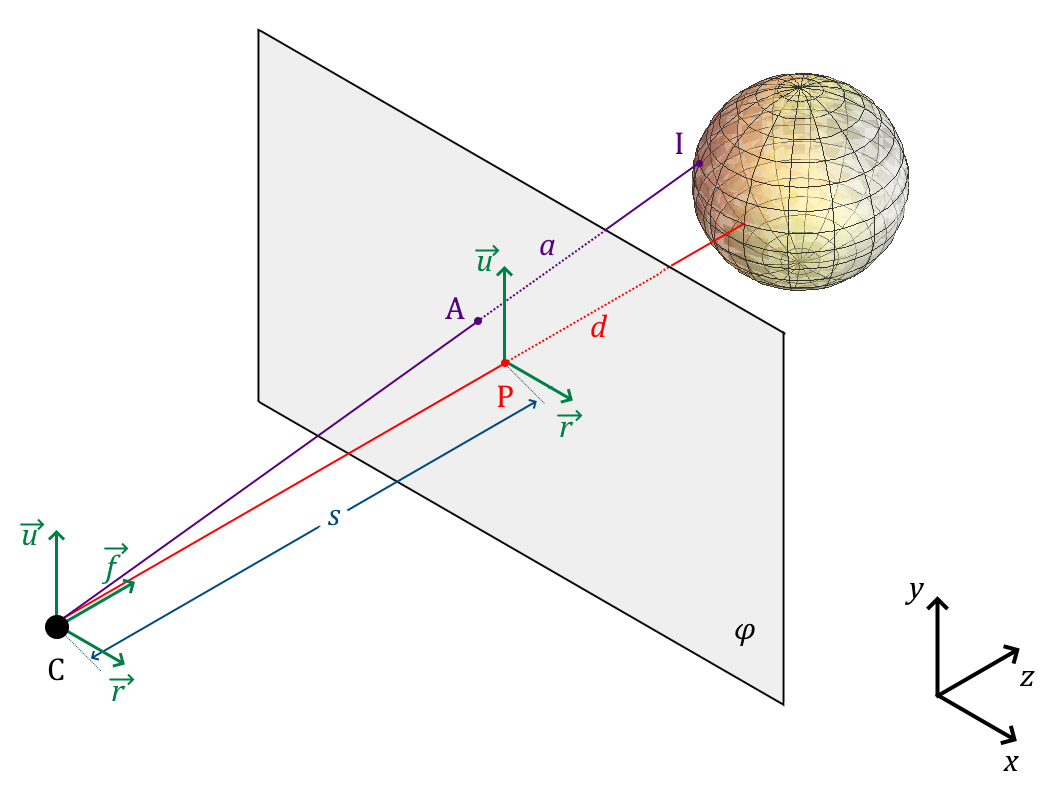
\includegraphics[width=\textwidth]{raycast}
	\caption[Esquema do processo de \textit{ray casting}]{Esquema representativo do processo de \textit{ray casting}. A partir do observador $C$, com os respetivos vetores de visualização $\overrightarrow{f}$, $\overrightarrow{r}$ e $\overrightarrow{u}$, e o \acs{FOV} definido pela distância $s$, determina-se o plano de visualização $\varphi$. Os raios emitidos, $a$, interceptam $\varphi$ no ponto $A$, o qual está associado a um fragmento no \opengl.}
	\label{fig::raycast}
\end{figure}

O ponto $P$ a partir do qual se definirá o plano de visualização é definido por:

\begin{equation}
	P = C + s \cdot \overrightarrow{f}
	\label{eq::cast:pontoP}
\end{equation}

Desta forma, o \textbf{plano de visualização} $\varphi$ é definido com base no ponto $P$ e nos vetores $\overrightarrow{r}$ e $\overrightarrow{u}$:

\begin{equation}
	\varphi ~\equiv~ (x,y,z) = P + x \cdot \overrightarrow{r} + y \cdot \overrightarrow{u}
	\label{eq::cast:plano}
\end{equation}

Desta forma, os \textbf{raios} emitidos a partir do observador, $a$, interceptam o plano de visualização $\varphi$ no ponto $A(x_A, y_A, z_P)$, e são definidos pela seguinte equação vetorial:

\begin{equation}
	a ~\equiv~ (x,y,z) = C + w \cdot (A - C)
	\label{eq::cast:ray}
\end{equation}

Através de um processo de \textit{ray marching} pode-se estimar o valor $w$ que determina o ponto de intercepção $I$. A distância a que se encontra do observador, em conjunto com o vetor normal em $I$, permitem calcular a cor do fragmento (geralmente um pixel) associado ao ponto $A$.


\subsection{Algoritmo naïve}
\label{ssec::art:raymarch:naive}

% Em \textit{ray tracing} apenas nos focamos na interseção do raio emitido com a superfície, enquanto no algoritmo de \textit{ray marching} marchamos na direção tomada até encontrarmos uma interseção (isto se a mesma existir).

No algoritmo naïve, um ponto é iterado sobre o raio emitido num processo de ``marcha''. A cada ponto o valor da função implícita é calculado. Assumindo que esta é contínua em $\mathbb{R}^3$, o Teorema de Bolzano-Cauchy pode ser utilizado para determinar se ocorreu uma interseção entre dois pontos de marcha contíguos (Figura \ref{fig::rmarching2D}).

\begin{figure}[!bp]
	\centering
	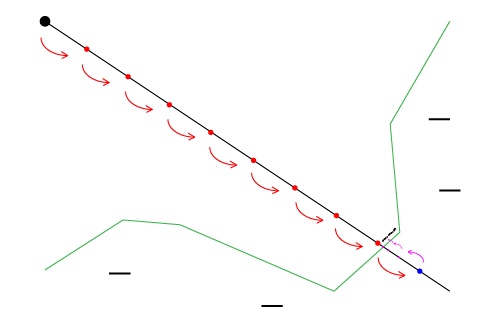
\includegraphics[width=.9\textwidth]{raymarch2D}
	\caption[Algoritmo \textit{Ray Marching} em 2D]{Demonstração do algoritmo \textit{Ray Marching} em 2D. Um ponto (a vermelho) ``marcha'' ao longo de um raio emitido no sentido da cena com origem no observador até ser detetada uma interseção com a função implícita (verde). O Teorema de Bolzano-Cauchy indica que tal interseção existe entre o último ponto vermelho e o ponto azul.}
	\label{fig::rmarching2D}
\end{figure}

A fim de aumentar a precisão do ponto de interseção estimado, pode-se proceder a uma marcha em sentido inverso com distâncias menores a cada iteração até se chegar a um ponto suficientemente perto da função implícita que se possa considerar o ponto de interseção. A este processo dá-se o nome de \textit{bisection} (Figura \ref{fig::rmarching2DBisection}).

Esta técnica é de particular interesse nos seguintes casos:
\begin{itemize}
    \item Necessidade de renderizar volumes que não são uniformes;
    \item Renderização de funções implícitas ou fractais;
    \item Renderização de outros tipos de funções paramétricas onde a interseção não é conhecida antecipadamente, como \textit{parallel mapping}.
\end{itemize}

Contudo, este é um algoritmo geral que se pode aplicar a qualquer função tridimensional (Figura \ref{fig::ashalgosphere}).

\begin{figure}[!htbp]
    \centering
    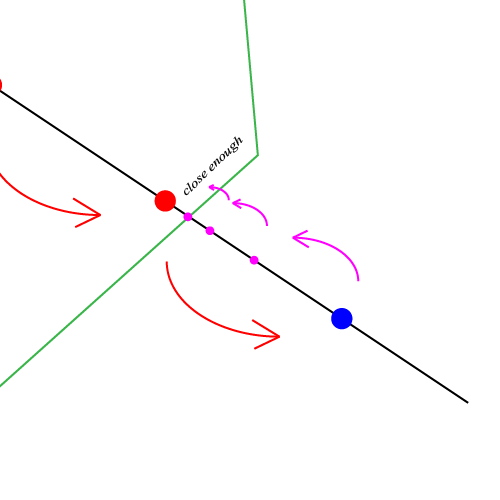
\includegraphics[width=0.8\textwidth]{bisection}
    \caption[Processo de \textit{bisection} usado no algoritmo naïve de \textit{ray marching}]{Processo de \textit{bisection} usado no algoritmo naïve de \textit{ray marching}.}
    \label{fig::rmarching2DBisection}
\end{figure}

\begin{figure}[!htbp]
	\centering
	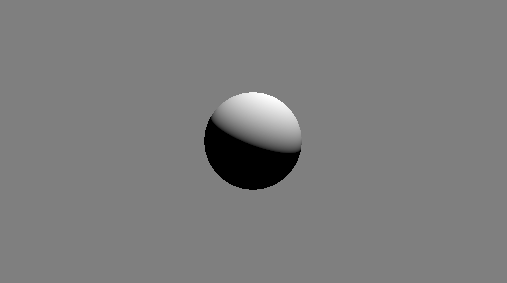
\includegraphics[width=0.6\textwidth]{ashalgosphere}
	\caption[Teste do algoritmo naïve numa esfera]{Teste do algoritmo naïve no \textit{website} \url{shadertoy.com} com uma esfera.}
	\label{fig::ashalgosphere}
\end{figure}

%\begin{algorithm}[!htbp]
%	\caption{Algoritmo naïve de \textit{ray marching}.}
%	\label{alg::raymarch_naive}
%	\begin{algorithmic}
%\Require função $f$      \Comment{Função implícita}
%	\end{algorithmic}
%\end{algorithm}


\subsection{\textit{Sphere Tracing}}
\label{ssec::arte:raymarch:spheretracing}

\textit{Sphere tracing} é uma técnica que faz uso do algoritmo de \textit{ray marching} para renderizar \textbf{superfícies implícitas} conhecidas (Figura \ref{fig::spheresphere}). É \textbf{requisito necessário} ter conhecimento antecipado da distância mínima entre um dado ponto e a superfície em questão. Esta distância é determinada com funções denominadas de \textbf{\ac{SDF}} (Figura \ref{fig::sdf}). O uso das mesmas torna impraticável a aplicação de \textit{sphere tracing} para funções implícitas de geometria desconhecida.

Visto que uma função \acs{SDF} pode ser resolvida para cada ponto, podemos determinar a maior esfera possível que possa caber no atual passo de marcha e cujo raio seja a distância mínima entre o ponto e a superfície. Sabemos então que a próxima distância a ``marchar'' é o raio desta esfera (Figura \ref{fig::stracing2D}). Tal permite optimizar o número de passos necessário na ``marcha'', aumentando significativamente a eficiência do processo de \textit{ray marching}.

%\begin{algorithm}[!htbp]
%	\caption{Algoritmo de \textit{sphere tracing}.}
%	\label{alg::raymarch_spheretrace}
%	\begin{algorithmic}
%		\Require função $f$      \Comment{Função implícita}
%	\end{algorithmic}
%\end{algorithm}

\begin{figure}[!htbp]
	\centering
	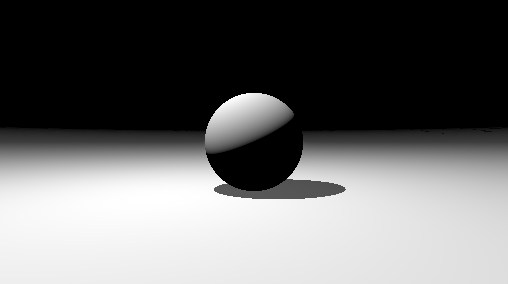
\includegraphics[width=0.6\textwidth]{spheresphere}
	\caption[Teste do algoritmo de \textit{sphere tracing}]{Teste do algoritmo de \textit{sphere tracing} no \textit{website} \url{shadertoy.com} de uma esfera e um plano.}
	\label{fig::spheresphere}
\end{figure}

\begin{figure}[!htbp]
	\centering
	
\includegraphics[width=0.4\textwidth]{sdf02}
	\caption[\acs{SDF} para a circunferência $x^2 + y^2 - 1$]{Visualização da \acf{SDF} para a circunferência $x^2 + y^2 - 1$. A escala de cinzas é proporcional à distância à superfície, sendo preto em valores negativos.}
	\label{fig::sdf}
\end{figure}

\begin{figure}[!htbp]
	\centering
	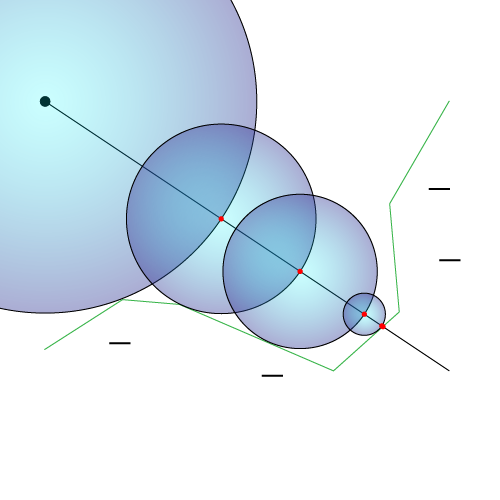
\includegraphics[width=0.8\textwidth]{stracing2D}
	\caption[Algoritmo de \textit{Sphere Tracing} em 2D]{Demonstração do algoritmo \textit{Sphere Tracing} em 2D. Cada novo ponto de ``marcha'' é distancia-se do anterior a uma distância igual ao raio da esfera que satisfaz a função \acs{SDF} para a superfície visualizada.}
	\label{fig::stracing2D}
\end{figure}


\section{\opengl}
\label{sec::arte:opengl}

Pela década de 80, o processo de desenvolvimento de \textit{software} que funciona-se em diferentes tipos de \textit{hardware} gráfico era algo desafiador pela grande falta de \textit{standards}. No inicio da década seguinte, \textit{Silicon Graphics} (SGI) era a atual líder em \textit{workstations} de gráficos 3D. E o seu \textit{IRIS GL} tornou-se o \textit{standard} na industria.

Entretanto apareceu o \opengl como uma alternativa ao \textit{IRIS GL}, uma \ac{API} que nos providencia um vasto conjunto de funcionalidades que podemos usar para manipular imagens e gráficos. Por si só \opengl não é apenas uma \ac{API}, mas sim uma especificação. Desenvolvida e mantida pela \textit{Kronos Group}, é encarregue de especificar o resultado de cada função e como a mesma se deve comportar para um determinado \textit{hardware}.

\opengl é no fundo uma grande \textbf{\textit{state machine}}: uma coletânea de variáveis que descreve como o \opengl se deverá comportar no momento. Durante o seu uso mudamos o seu estado definindo algumas opções, alguns \textit{buffers} e então renderizando usando o atual contexto.

\subsection{\textit{Pipeline}}
\label{ssec::arte:opengl:pipeline}

A renderização de um dado objeto em \opengl~passa por diversos passos, a cujo conjunto é dado o nome de \textbf{\textit{pipeline} de renderização}. A partir da versão 3.3, intitulado de ``\opengl moderno'', a \textit{pipeline} possui determinados pontos onde o programador tem a capacidade de programar diretamente para a \ac{GPU} através de pequenos programas compostos por \textit{shaders}.

A \textit{pipeline} é executada sempre que uma operação de renderização for iniciada. Estas operações requerem o uso obrigatório de um \ac{VAO} propriamente definido, em conjunto com um \textit{Program Object} ou um \textit{Program Pipeline Object}, o qual fornece os \textit{shaders} para certos pontos da \textit{pipeline}.

Das fases englobadas pela \textit{pipeline}, destacam-se cinco:

\begin{enumerate}
    \item \textbf{Processamento de vértices} (\textit{vertex processing}):
    Esta fase é programável em três pontos consecutivos, o que abre uma vasta margem de customização ao programador sobre como os vértices são processados.
    Após a especificação do vértice, este é processado por um \textit{vertex shader} tornando-o num vértice de saída. Opcionalmente pode-se manipular o processo seguinte, de tesselação (\textit{tessellation stage}), assim como processamento de primitivas com o uso de um \textit{geometry shader}, igualmente opcional.
    
    \item \textbf{Pós-processamento de vértices} (\textit{vertex post-processing}):
    Durante este processo os vértices disponíveis são filtrados pela condição de serem compreendidos no \textit{viewport} atual. Os mesmos também poderão ser transportados para diferentes localizações no espaço.
    
    \item \textbf{Rasterização} (\textit{rasterization}):
    É neste processo que as primitivas são divididas em elementos independentes designados de \textbf{fragmentos}. Por norma, a cada pixel é associado um fragmento.
    
    \item \textbf{Processamento de Fragmentos}:
    Para cada fragmento é gerado uma quantia de \textit{outputs} (por exemplo a cor), processados por um \textit{fragment shader}, cuja customização pelo programador é opcional.
    
    \item \textbf{Processamento por Amostra} (\textit{per-sample operations}): Com os resultados devolvidos pelo \textit{fragment shader}, os mesmos passam por diversos testes (por exemplo, de profundidade), resultando então num pixel final.
\end{enumerate}


\subsection{\textit{Shaders}}
\label{ssec::arte:opengl:shaders}

Aos sub-programas executados pela \ac{GPU} num determinado ponto da \textit{pipeline} de renderização chamamos de \textit{shaders}. Um conjunto de \textit{shaders} constitui um \textbf{programa}. Por entre os diversos \textit{shaders} disponíveis para implementação, são destacados dois de interesse a este projeto:

\begin{enumerate}
    \item \textbf{\itshape Vertex Shader}:
    Recebendo como \textit{input} um vértice no espaço, este \textit{shader} é usado no processamento de vértices. Tradicionalmente realiza operações matriciais \ac{MVP}. É o único \textit{shader} cuja presença é \textbf{obrigatória} num programa.
    
    \item \textbf{\itshape Fragment Shader}:
    Recebendo um fragmento após o processo de rasterização como \textit{input}, o \textit{fragment shader} é capaz de o processar a fim de devolver uma determinada cor em conjunto com uma profundidade. Tradicionalmente, é neste \textit{shader} que são aplicadas operações de iluminação e coloração.
\end{enumerate}

Os \textit{shaders} são compilados em \textit{runtime} pelo \opengl. Estes são implementados numa linguagem própria, com sintaxe próxima à linguagem \verb|C|, denominada \acf{GLSL}.

É possível enviar uma cópia de dados da \ac{CPU} para a \ac{GPU} com recurso a \textbf{variáveis uniformes} (\textit{uniforms}). Estas funcionam como variáveis globais em qualquer \textit{shader}. No entanto, dados relativos a vértices, normais e cores são passados por \textbf{\textit{buffers}}.


\subsection{\textit{Vertex Attribute Object}}
\label{ssec::arte:opengl:vao}

Com a finalidade de passar diversos dados para a \ac{GPU}, é obrigatório usar um gestor de atributos denominado por \acf{VAO}. Este é geralmente usado para organizar atributos de diversos \textit{buffers} (e.g. \ac{VBO} e \ac{CBO}).

Tendo em conta que o mesmo é mandatório na execução da \textit{pipeline}, e não havendo a necessidade de alocar \textit{buffer objects}, é possível fornecer à \ac{GPU} um \ac{VAO} pré-definido:

\begin{minted}[linenos]{c++}
    unsigned int vaoHandle;
    glGenVertexArrays(1, &vaoHandle);
    glBindVertexArray(vaoHandle);
    glVertexAttrib1f(0, 0);
    glBindVertexArray(0);
\end{minted}

% Desta forma é possível iniciar a execução da \textit{pipeline} de renderização sem fornecer \textit{buffer objects}.


%\subsection{Texturas}
%\label{ssec::arte:opengl:texturas}
%\todo{}


%\section{Conclusões}
%\label{sec::arte:conc}
